\section{Records}


\subsection{template}

\subsubsection{实验目的}


\subsubsection{实验信息}


\begin{table}[H]
	\centering
	\begin{spacing}{1.5}
	\begin{tabular}{cc}\hline
		实验特征 & 实验信息 \\
		\hline
		实验编号 & \\
		实验日期 &  \\
		实验者 & \\
		实验设备& \\
		输出文件地址 & \\
		Git 信息 & \\
		Ex\_key & \\
		模型文件地址 & \\
		训练文件地址 & \\
		关键信息 & \\\hline
	\end{tabular}
	\end{spacing}
\end{table}


\subsubsection{实验结果}


\begin{enumerate}[1.]
	\item \textbf{稳定性评价:}
	\item \textbf{精度评价:}
\end{enumerate}


\subsubsection{实验分析}


\subsubsection{实验计划}

\newpage



\subsection{2022-03-14}\label{subsec:03-14}

\subsubsection{实验目的}

在前面的实验(2022-3-14-New)中,虽然我们能从注意力中获得的分割结果较为精确,但是我们发现CycleGAN会在\replace{epoch}{iter}为2000附近时会出现模式崩溃现象,即所有的Attention都为零,网络不再训练。我猜测是因为判别器的学习率过大的原因导致的,所以在这一次实验中将判别器的学习率由2e-3降低为2e-4,生成器的学习率2e-3保持不变,但依然遵循学习率策略,希望以此来解决\colorbox{yellow}{模式崩溃问题}。

\subsubsection{实验信息}


\begin{table}[H]
	\centering
	\begin{spacing}{1.5}
		\begin{tabular}{cc}\hline
			实验特征 & 实验信息 \\
			\hline
			实验编号 & CC-LY-2022-03-14-A\\
			实验日期 &  2022-03-14\\
			实验者 & 刘烨\\
			实验设备 & 3080Ti\\
			输出文件地址 & 2022-03-14-18-57-01.152050\\
			Git 信息 & 2022-3-14-New\\
			模型文件地址 & checkpoints\\
			训练文件地址 & settings.yml\\
			关键信息 & \underline{\textbf{往稳定的方向发展}}\\\hline
		\end{tabular}
	\end{spacing}
\end{table}


\subsubsection{实验结果}


\begin{figure}[H]
	\centering
	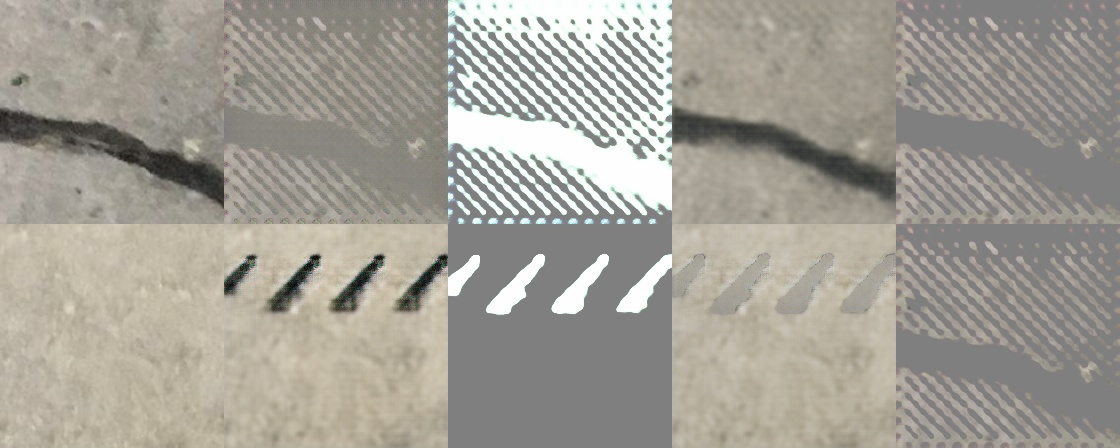
\includegraphics[width=240pt,height=110pt]{0314//iter-000002300}
	\caption{iter-000002300.jpg}
\end{figure}
\begin{figure}[H]
	\centering
	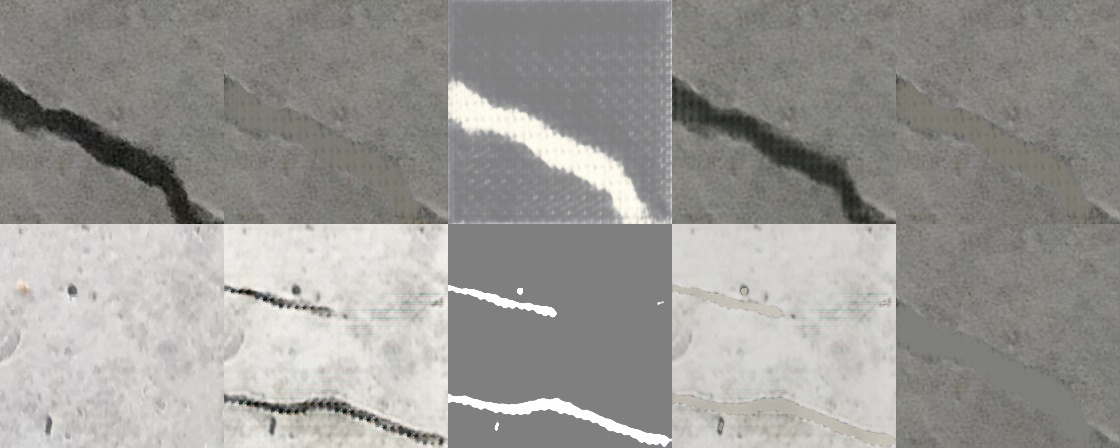
\includegraphics[width=240pt,height=110pt]{0314//iter-000016000}
	\caption{iter-000016000.jpg}
	\label{fig:fig.2}
\end{figure}
\begin{figure}[H]
	\centering
	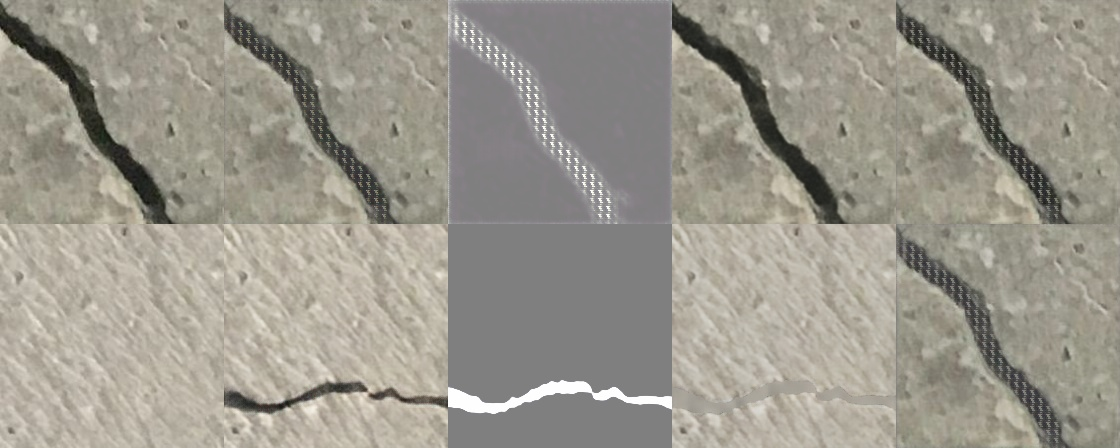
\includegraphics[width=240pt,height=110pt]{0314//iter-000060600}
	\caption{iter-000060600.jpg}
\end{figure}


\subsubsection{实验分析}

从实验的三个阶段来看,实验在稳定性与准确性上有了较大的提升。稳定性是指整个网络完成了10个epoch的19000张图片训练,并且最终还能维持良好的效果。
准确性是指整个网络在分割的精细化相比之前较为模糊的结果有了较大的提升。但是仔细的来看的话,分割结果出现明显的点状噪音,致使分割的精度达不到
有监督网络的要求。然后从还原的Mask——$input * (1 - attention)$ 来看,其还原效果并没有真正地与输出$h$区分开,这两者的相似度甚至非常之高,
需要进一步找到原因。还有一个值得关注的点就是在无裂缝图像这一循环中,它的转换效果与分割效果都是极佳的,非常符合设计预期,如何在有裂缝图像中复现这
种模式呢?值得思考。

\subsubsection{实验计划}

下一步计划针对网络中的输出进行研究,将还原Mask与Content Mask修改为设想的状况,目前实验设计方向:
\begin{enumerate}[1.]
	\item 参照AttentionGAN v2中的架构对模型进行后半段的修改,输出Head不发生改变。
	\item 保持现有模型结构不变,针对输出Head进行调整,主要是针对其中的关系进行分析,考虑加入\colorbox{yellow}{自监督}的方法。
\end{enumerate}

\subsubsection{关键实验小结}
\begin{enumerate}[1.]
	\item 调整 $D$ 与 $G$ 的学习率,从而使两者达到平衡,取得不错的效果。
	\item 加入SSIM结构相似度控制函数,提升分割精度,但模型设计仍不完善。
	\item 无裂缝循环段实验效果良好。
\end{enumerate}
\newpage


\subsection{2022-03-19}\label{subsec:03-19}

\subsubsection{实验目的}

这个实验承接实验\ref{subsec:03-14} 的思路,同时融合AttentionGAN\_v2的思路。因为实验\ref{subsec:03-14} 中的网络中的Content与
Attention承接下采样之后的特征层,此时特征层的信息可能趋于同一化,无法真正地将Content与Attention之间的差异表示出来,导致网络的几个输出信息
差异性较小,偏离预想结果。故针对网络模型进行修改,观察其输出,预期网络参数会增加不少,网络输出信息之间的差异性表现更加明显,分割精度得到提升。

\subsubsection{实验信息}


\begin{figure}[H]
	\centering
	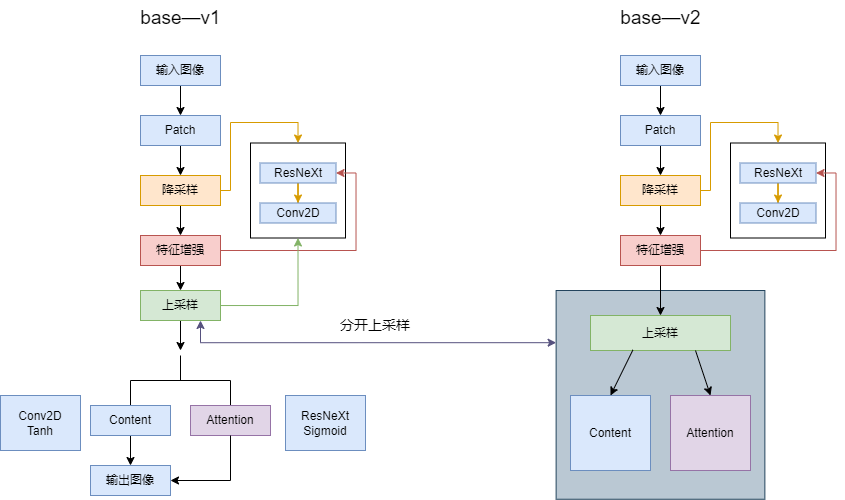
\includegraphics[width=338pt,height=200pt]{0319//03-14-AttentionGAN_base}
	\caption{网络模型变更示意图}
\end{figure}


\begin{table}[H]
	\centering
	\begin{spacing}{1.5}
		\begin{tabular}{cc}\hline
			实验特征 & 实验信息 \\
			\hline
			实验编号 & 2022-03-19-AttentionGAN\_v2\_Base\\
			实验日期 & 2022-03-19 \\
			实验者 & 刘烨\\
			实验设备& 3080Ti\\
			输出文件地址 & 2022-03-19-18-41-23.687397\\
			Git 信息 & 2022-03-19-AttentionGAN\_v2\_Base\\
			Ex\_key & f82d954af7fd41aa8cb069f69fb3a23f\\
			模型文件地址 & module\_code\\
			训练文件地址 & hyper\_params.json\\
			关键信息 & \colorbox{red!40}{分割结果精细化问题与稳定性问题}\\\hline
		\end{tabular}
	\end{spacing}
\end{table}


\subsubsection{实验结果}

\begin{figure}[H]
	\centering
	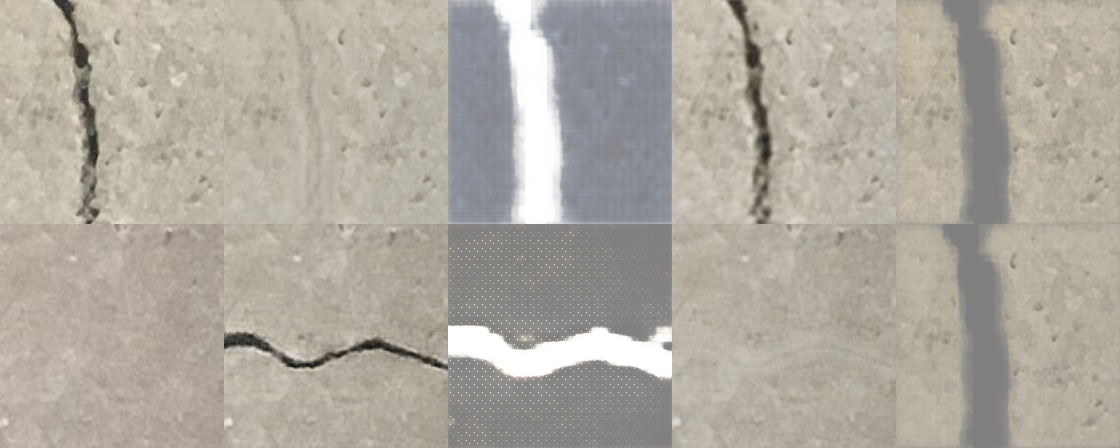
\includegraphics[width=240pt,height=110pt]{0319//iter-000019900}
	\caption{iter-000019900.jpg}
	\label{fig:fig.5}
\end{figure}
\begin{figure}[H]
	\centering
	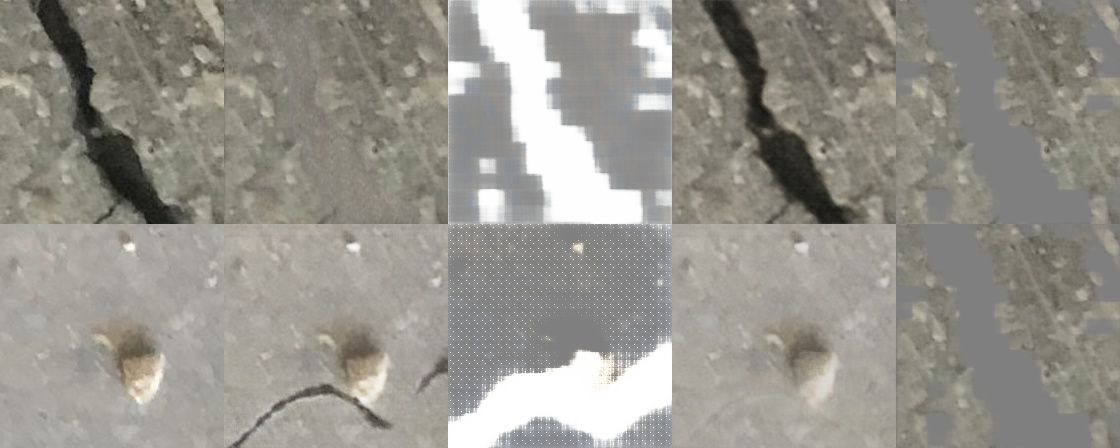
\includegraphics[width=240pt,height=110pt]{0319//iter-000057400}
	\caption{iter-000057400.jpg}
	\label{fig:fig.6}
\end{figure}
\begin{figure}[H]
	\centering
	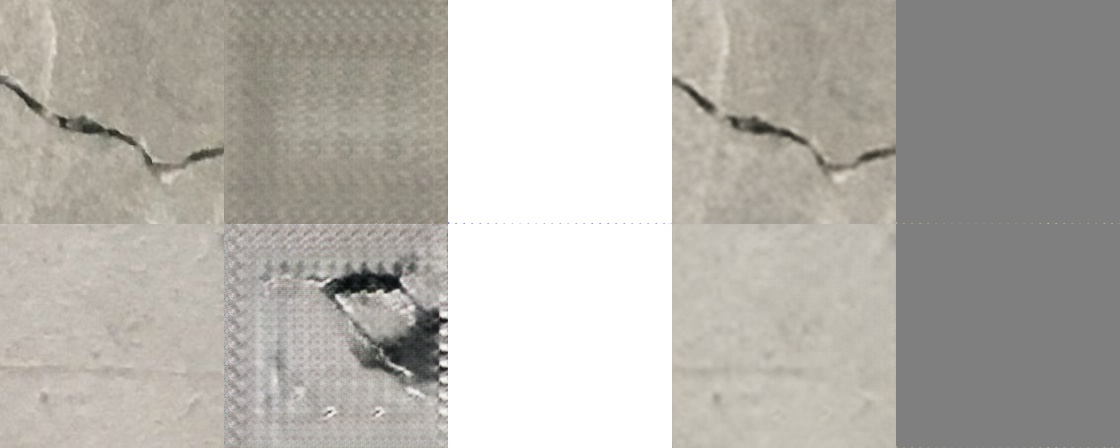
\includegraphics[width=240pt,height=110pt]{0319//iter-000091900}
	\caption{iter-000091900.jpg}
\end{figure}


\begin{enumerate}[1.]
	\item \textbf{稳定性评价:} 40分,在训练后期趋于崩溃
	\item \textbf{精度评价:} 40分,分割结果太保守,不够精细
\end{enumerate}


\subsubsection{实验分析}

再进行了模型改动之后,ssim图像的输出结果符合了预期,可以从图像\ref{fig:fig.5} 与图像\ref{fig:fig.6}
中可以看到,它正确地将这一部分掩盖掉了,但是回过头去观察\ref{subsec:03-14} 的实验结果发现图像\ref{fig:fig.2}
的结果甚至比现在的还要精确,有点\colorbox{red!40}{疑惑}之前提到的不符合是什么意思?有点不太记得了。然后从裂缝图像到
无裂缝图像这一循环的分割结果来看,分割结果非常差,粒度非常大,并且噪点也非常多。从无裂缝向有裂缝图像循环中也是如此,粒度非常大,
远没有\ref{subsec:03-14} 实验中的那么精细。最后,在实验的后期,该网络趋于崩溃,实验结果非常不好。预期是因为使用两个上采样块
使得两者的信息出现了较大的偏离,可能并不需要使用复杂的Double Heads上采样块,因为它没有监督信息去约束它。

\subsubsection{实验计划}

对\ref{subsec:03-14} 进行重新实验,目前猜测\ref{subsec:03-14} 实验的模型更加符合预期,应该在此模型上做出改进。

\newpage

\subsection{03-19-B}\label{subsec:03-19-b}

\subsubsection{实验目的}

针对\ref{subsec:03-19} 中出现的严重模式崩溃问题,本实验在损失函数设计上进行了修改,修改了ssim\_loss\_3,使其与原始图像满足相似性约束,从而使其生成高质量的图像。

\subsubsection{实验信息}


\begin{table}[H]
	\centering
	\begin{spacing}{1.5}
		\begin{tabular}{cc}\hline
			实验特征 & 实验信息 \\
			\hline
			实验编号 & AttentionGAN\_v2\_Base\_B\\
			实验日期 &  2022-03-19\\
			实验者 & 刘烨\\
			实验设备& 3090\\
			输出文件地址 & 2022-03-19-22-15-21.477612\\
			Git 信息 & AttentionGAN\_v2\_Base\_A\\
			Ex\_key & 23ef86bffc0d4ea59057c2681f95faf3\\
			模型文件地址 & module\_code\\
			训练文件地址 & summaries\\
			关键信息 & \colorbox{red!40}{分割结果精细化问题}\\\hline
		\end{tabular}
	\end{spacing}
\end{table}


\subsubsection{实验结果}

\begin{figure}[H]
	\centering
	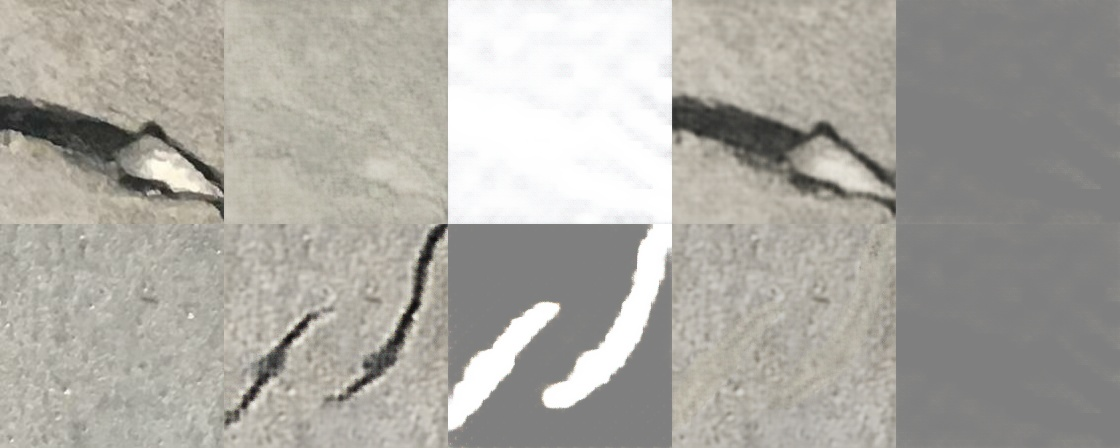
\includegraphics[width=240pt,height=110pt]{0319//iter-000006700}
	\caption{iter-000006700.jpg}
\end{figure}
\begin{figure}[H]
	\centering
	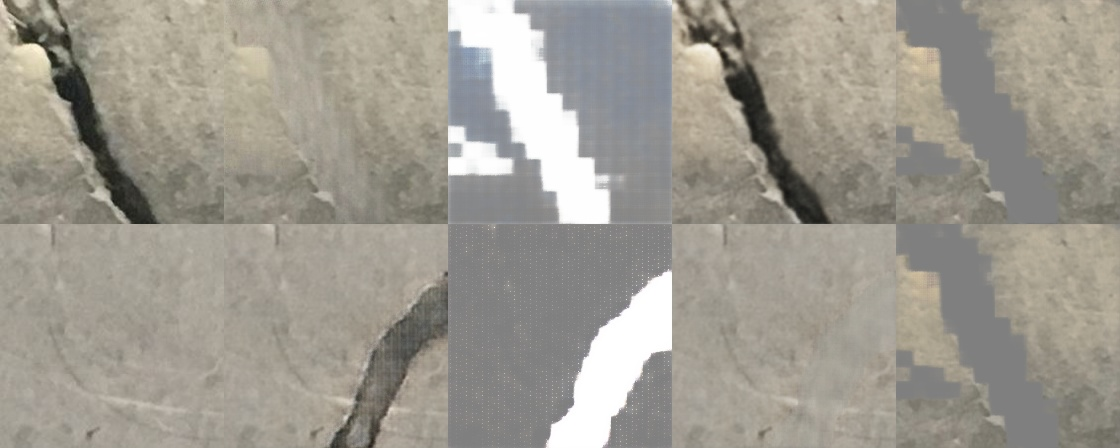
\includegraphics[width=240pt,height=110pt]{0319//iter-000041200}
	\caption{iter-000041200.jpg}
\end{figure}
\begin{figure}[H]
	\centering
	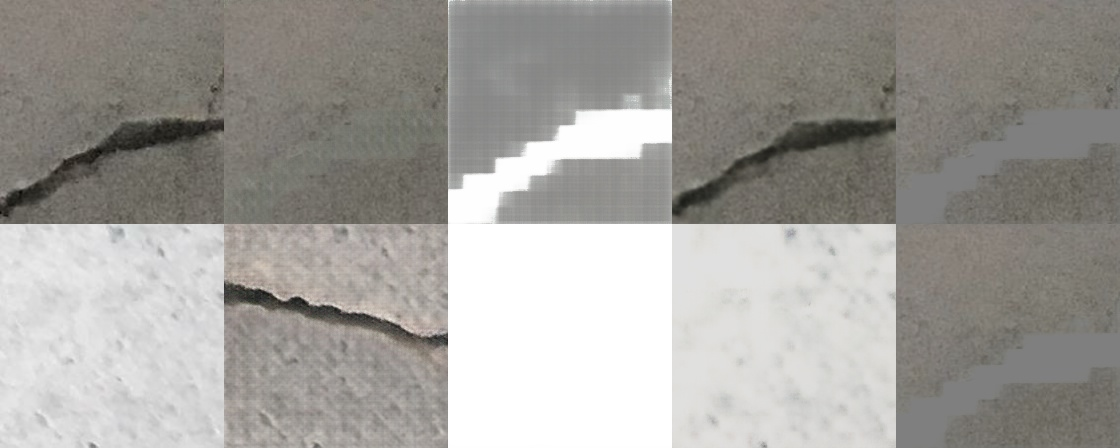
\includegraphics[width=240pt,height=110pt]{0319//iter-000089300}
	\caption{iter-000089300.jpg}
\end{figure}

\begin{enumerate}[1.]
	\item \textbf{稳定性评价:} 60分, 与\ref{subsec:03-19} 实验相比,实验末期没有出现崩溃现象,但结果依然不稳定。
	\item \textbf{精度评价:} 40分,与\ref{subsec:03-19} 实验一样,分割精度过低,估计是AttentionGAN\_v2模型的问题。
\end{enumerate}


\subsubsection{实验分析}

估计是模型本身的问题,预期舍弃AttentionGAN\_v2模型。

\subsubsection{实验计划}

重新跑一下AttentionGAN\_v1模型再次观察其性能表现。
\begin{enumerate}[1.]
	\item \textbf{模型修改:} 针对AttentionGAN\_v1模型进行改进式修改。
	\item \textbf{替换新模型:} 适应CAM类激活图进行训练。
	\item \textbf{文献阅读:} Label4Free模型启发。
\end{enumerate}

\newpage

\subsection{03-20}

\subsubsection{实验目的}

根据实验\ref{subsec:03-19}与\ref{subsec:03-19-b}两个实验的实验结果来看,AttentionGAN\_v2并不是合适的网络模型,所以回滚到\ref{subsec:03-14}
再次运行 AttentionGAN 观察其稳定性如何,实验产生的随机性大吗?如果模型表现良好,可考虑在此模型上进行优化。目的为复现
AttentionGAN,观察其稳定性与精度,其结果应该与\ref{subsec:03-14} 实验结果相类似。

\subsubsection{实验信息}


\begin{table}[H]
	\centering
	\begin{spacing}{1.5}
		\begin{tabular}{cc}\hline
			实验特征 & 实验信息 \\
			\hline
			实验编号 & AttentionGAN\_Base\_Repeat\\
			实验日期 &  2022-03-20\\
			实验者 & 刘烨\\
			实验设备& 3090\\
			输出文件地址 & E:/Cycle\_GAN/output/2022-03-20-23-30-36.135129\\
			Git 信息 & 03--20 AttentionGAN\_Base\_Repeat\\
			Ex\_key & 2d978edbb82f4da9a9f1793430e4a9c1\\
			模型文件地址 & module\_code\\
			训练文件地址 & summaries\\
			关键信息 & \underline{\emph{基本稳定}}\\\hline
		\end{tabular}
	\end{spacing}
\end{table}


\subsubsection{实验结果}

\begin{figure}[H]
	\centering
	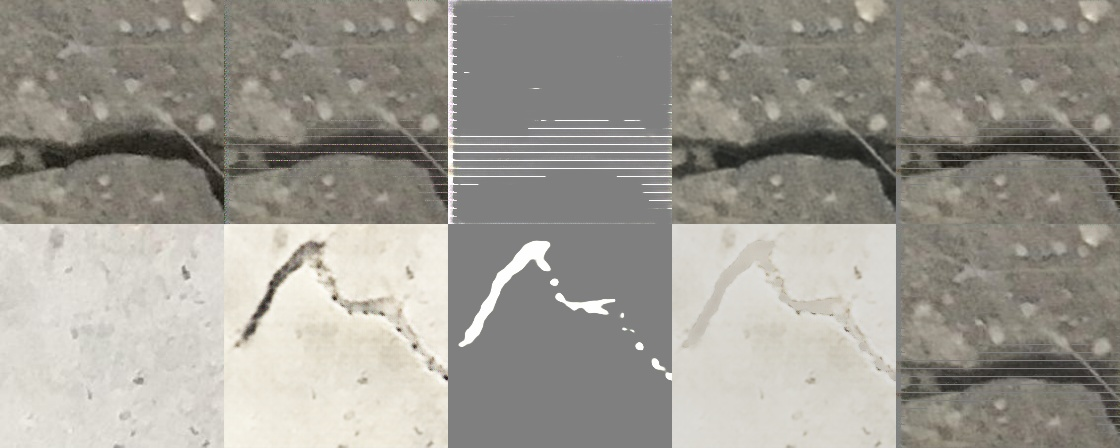
\includegraphics[width=240pt,height=110pt]{0320//iter-000020000}
	\caption{iter-000020000.jpg}
\end{figure}
\begin{figure}[H]
	\centering
	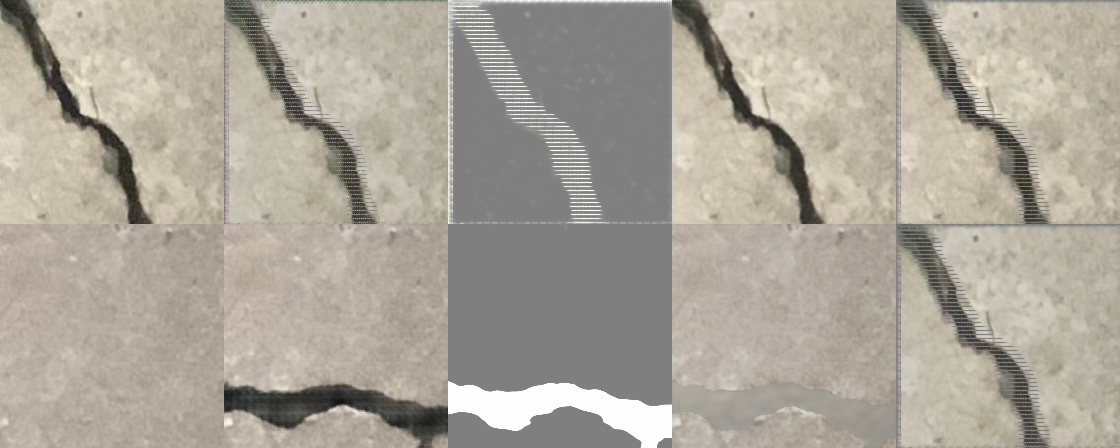
\includegraphics[width=240pt,height=110pt]{0320//iter-000047100}
	\caption{iter-000047100.jpg}
\end{figure}
\begin{figure}[H]
	\centering
	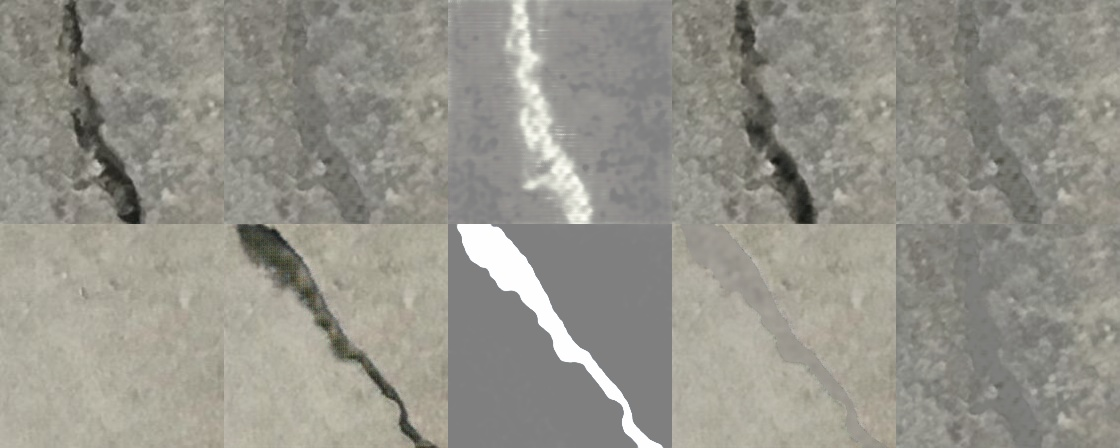
\includegraphics[width=240pt,height=110pt]{0320//iter-000075100}
	\caption{iter-000075100.jpg}
\end{figure}

\begin{enumerate}[1.]
	\item \textbf{稳定性评价:} 60分,稳定性基本满足要求,但是输出的注意图容易缺少信息,模糊并且图像边缘常存在。
	\item \textbf{精度评价:} 50分, 与之前的AttentionGAN结果相似,容易出现模糊。——是不是不需要训练那么多次呢?
\end{enumerate}


\subsubsection{实验分析}

AttentionGAN是相对比较稳定的模型的,但是精度还需要继续增加。

\subsubsection{实验计划}

\paragraph{\textbf{模型修改:}}
\begin{enumerate}[1.]
	\item 针对AttentionGAN\_v1模型进行改进式修改。
	\item 删除了ssim\_loss\_3
	\item 增加了方差损失函数
	\item 删除判别器B只保留判别器A
	\item 修改优化器RMSProp
	\item 调整判别器B的学习率
\end{enumerate}
\begin{figure}
	\centering
	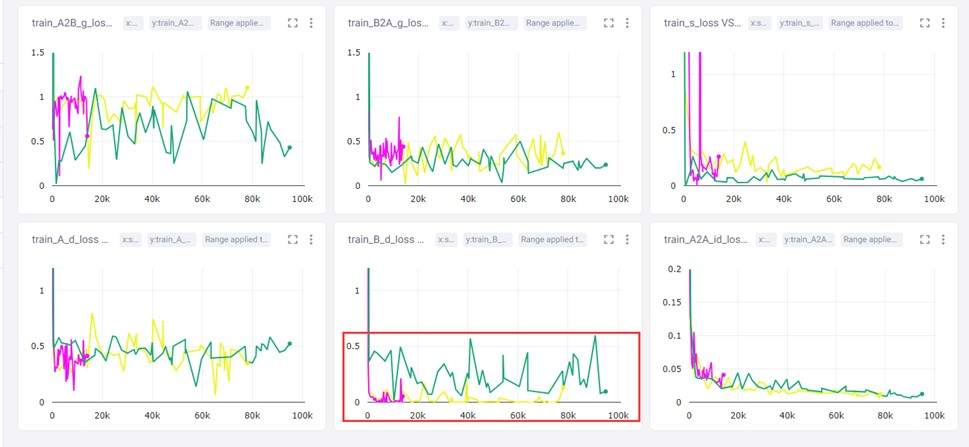
\includegraphics[width=360pt,height=160pt]{0320//1}
	\caption{iter-000020000.jpg}
\end{figure}
以上所有计划基本上全部失败
另外我观察到,是不是对于生成模型,Batchsize越小越好呢?
然后是不是应该想一些其他正常的方式呢?没必要死磕GAN。



\newpage



\subsection{05-12}

\subsubsection{实验目的}

根据近两个月的实验与计算机视觉老师的补充,整体实验思路已经完成,目前进入到实验验证阶段。实验验证主要分三个数据集进行实验,此次为简单数据集的最佳性能测试实验,目的是寻找最佳的实验方案并保存。

\subsubsection{实验信息}


\begin{table}[H]
	\centering
	\begin{spacing}{1.5}
		\begin{tabular}{cc}\hline
			实验特征 & 实验信息 \\
			\hline
			实验编号 & 2022-05-12-A2A\_Weak\_D\_crack\_3080Ti \\
			实验日期 &  2022-05-12\\
			实验者 & 刘烨\\
			实验设备& 3080Ti\\
			输出文件地址 & E:/Cycle\_GAN/output/2022-05-12-11-11-39.737880/save\_model\\
			Git 信息 & 无\\
			Ex\_key & 6736db8b2430439a90d4109a0dd8ef4c\\
			模型文件地址 & 0-2700-0.8056701421737671\\
			训练文件地址 & E:/Cycle\_GAN/output/2022-05-12-11-11-39.737880/module\_code\\
			关键信息 & \textbf{SOTA 最好的模型-80.57\%}\\
			\hline
		\end{tabular}
	\end{spacing}
\end{table}


\subsubsection{实验结果}

\begin{figure}[h]
	\centering
	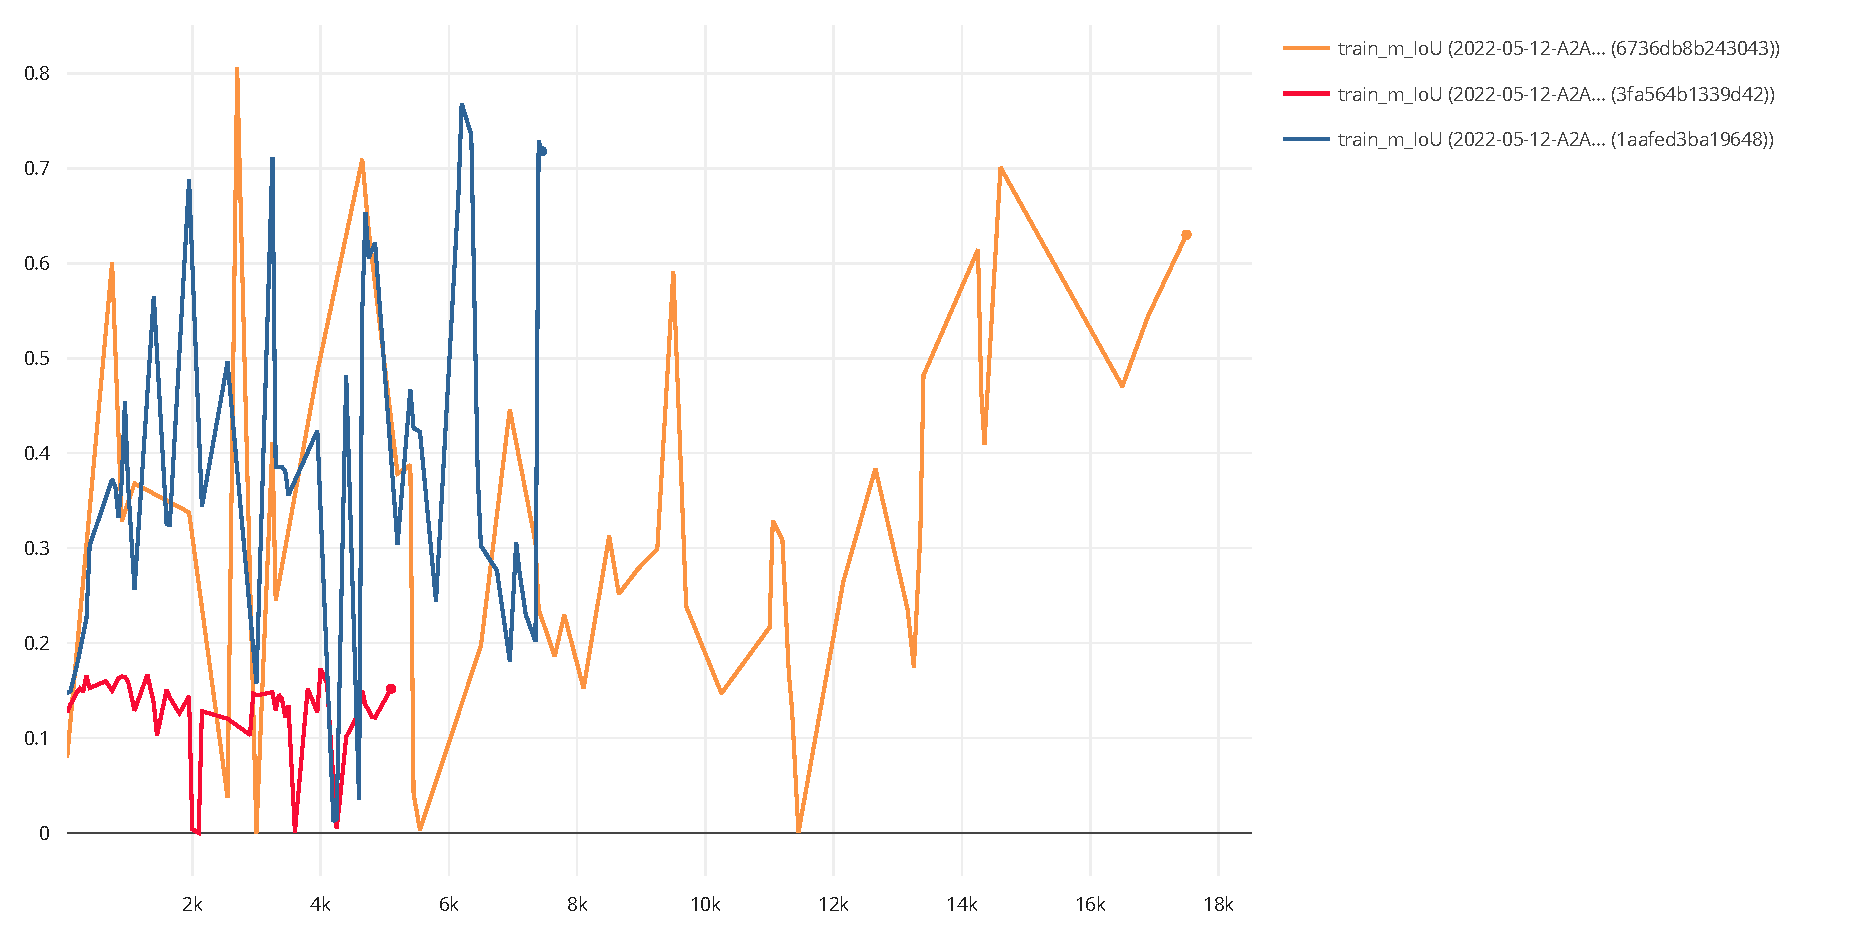
\includegraphics[width=360pt,height=160pt]{0512//1}
	\caption{CycleGAN\_for\_crack\_m\_IoU}
\end{figure}

\begin{enumerate}[1.]
	\item \textbf{稳定性评价:} 90分,实验结果可复现且在不同的设备上均表现稳定。
	\item \textbf{精度评价:} 100,简单数据集上的分割效果已经超过了经典有监督的分割网路。
\end{enumerate}


\subsubsection{实验分析}

本次实验一共使用了三个设备(3080Ti, 3090, 3090\_U), 结果有两点发现。

\subsubsection{实验计划}

\newpage